\documentclass[12pt, a4paper]{article}

% ==========================================
% 1. KHAI BÁO GÓI THƯ VIỆN (PACKAGES)
% ==========================================
% Bảng mã & Font chữ
\usepackage[utf8]{inputenc}
\usepackage[T5]{fontenc}

% Toán học
\usepackage{amsmath, amssymb}

% Căn lề & Bố cục trang
\usepackage[top=2.2cm, bottom=1.5cm, left=1cm, right=1cm, headheight=15pt]{geometry}
\usepackage{fancyhdr}
\usepackage{needspace}
\usepackage{tkz-tab}

% Đồ họa & Màu sắc
\usepackage{xcolor}
\usepackage{graphicx} 
\usepackage{tikz}
\usetikzlibrary{calc, shapes.geometric, positioning}


% Bảng biểu & Danh sách
\usepackage{colortbl}
\usepackage{array}
\usepackage{makecell}
\usepackage{multirow}
\usepackage{tasks}

% Biểu tượng
\usepackage{fontawesome5}

% ==========================================
% 2. THIẾT LẬP MÀU SẮC CHỦ ĐẠO
% ==========================================
\definecolor{goldyellow}{RGB}{255, 179, 0}
\definecolor{amberorange}{RGB}{230, 115, 0}
\definecolor{lightamber}{RGB}{255, 248, 225}
\definecolor{deepblue}{RGB}{25, 42, 86}
\definecolor{accentred}{RGB}{232, 65, 24}
\definecolor{softgray}{RGB}{220, 220, 222} 
\definecolor{fbblue}{RGB}{15, 80, 200}


% ==========================================
% 3. CẤU HÌNH HEADER & FOOTER
% ==========================================
\pagestyle{fancy}
\fancyhf{}
\renewcommand{\headrulewidth}{0pt}

% Khai báo biến lưu trữ nội dung góc phải của Header
\newcommand{\HeaderRightText}{}

% --- Header ---
\fancyhead[C]{
    \begin{tikzpicture}[remember picture, overlay]
        
        % Dải màu trang trí góc trên
        \path[fill=deepblue] (current page.north west) -- (current page.north east) 
            -- ($(current page.north east) + (0, -1.6cm)$) 
            .. controls ($(current page.north) + (3, -2.0cm)$) and ($(current page.north) + (-3, -0.4cm)$) .. 
            ($(current page.north west) + (0, -1.0cm)$) -- cycle;
            
        \path[fill=goldyellow] (current page.north west) -- (current page.north east) 
            -- ($(current page.north east) + (0, -1.0cm)$) 
            .. controls ($(current page.north) + (4, -1.0cm)$) and ($(current page.north) + (-2, -2.2cm)$) .. 
            ($(current page.north west) + (0, -1.6cm)$) -- cycle;
            
        \path[fill=amberorange] (current page.north west) -- ($(current page.north west) + (6.5cm, 0)$) 
            .. controls ($(current page.north west) + (4.5cm, -1.2cm)$) and ($(current page.north west) + (2cm, -2.0cm)$) .. 
            ($(current page.north west) + (0, -2.0cm)$) -- cycle;
            
        % Logo góc trái Header
        \node[anchor=west, inner sep=0pt] 
            at ($(current page.north west) + (0cm, -0.8cm)$) {
\includegraphics[height=2.0cm]{../../../image/logo-header.png}};
            
        % Text góc phải Header (Tự động lấy từ đối số thứ 3 của \titlebox)
        \node[anchor=east, text=white, font=\small\bfseries\sffamily] 
            at ($(current page.north east) + (-0.8cm, -0.5cm)$) {\HeaderRightText};
    \end{tikzpicture}
}

% --- Footer ---
\fancyfoot[C]{
    \begin{tikzpicture}[remember picture, overlay]
        % Đường kẻ ngang
        \draw[amberorange, line width=1.5pt] 
            ($(current page.south west) + (0cm, 0.4cm)$) -- ($(current page.south east) + (0cm, 0.4cm)$);

        % Dải cong góc phải
        \path[fill=goldyellow] (current page.south east) -- ($(current page.south east) + (-5cm, 0)$) 
            .. controls ($(current page.south east) + (-3cm, 0.8cm)$) and ($(current page.south east) + (-1.5cm, 1.2cm)$) .. 
            ($(current page.south east) + (0, 1.2cm)$) -- cycle;

        % Mạng xã hội
        \node[anchor=west, inner sep=0pt] at ($(current page.south west) + (1cm, 0.8cm)$) {
            \small\sffamily
            \textcolor{fbblue}{\faFacebook\hskip 4pt Toán Anh Huy MATH-STER}
            \hskip 18pt
            \textcolor{black}{\faTiktok\hskip 4pt huymathster}
        };

        % Số trang
        \node[circle, fill=white, draw=amberorange, line width=1.5pt, text=deepblue, font=\large\bfseries\sffamily, inner sep=4pt, minimum size=0.8cm] 
            at ($(current page.south east) + (-1.2cm, 0.6cm)$) {\thepage};
    \end{tikzpicture}
}

% ==========================================
% 4. ĐỊNH NGHĨA MACRO: KHUNG TIÊU ĐỀ
% ==========================================
\newcommand{\titlebox}[3]{
    % Gán nội dung đối số #3 vào biến HeaderRightText
    \gdef\HeaderRightText{#3}
    
    \begin{center}
    \vspace*{-0.5cm}
    \begin{tikzpicture}
        % Khung vô hình (Phantom Box) định chuẩn kích thước
        \node[text width=16cm, inner xsep=0pt, inner ysep=16pt, opacity=0] (MainBox) {
            \begin{minipage}[c]{4.2cm}
                \centering\vspace{0.1cm}
                \rule{2.2cm}{2.2cm} 
                \vspace{0.1cm}
            \end{minipage}%
            \begin{minipage}[c]{11.5cm}
                \centering\vspace{0.15cm}
                {\huge\bfseries\sffamily #2 \par}
                \vspace{0.15cm} 
            \end{minipage}
        };
        
        % Đổ bóng & Nền
        \fill[goldyellow, rounded corners=8pt] ([xshift=5pt, yshift=-5pt]MainBox.south west) rectangle ([xshift=5pt, yshift=-5pt]MainBox.north east);
        \fill[white, rounded corners=8pt] (MainBox.south west) rectangle (MainBox.north east);
        
        % Lưới ô ly & Nền Logo
        \begin{scope}
            \clip[rounded corners=8pt] (MainBox.south west) rectangle (MainBox.north east);
            \draw[step=0.4cm, softgray!50, line width=0.6pt] (MainBox.south west) grid (MainBox.north east);
            \fill[lightamber!60] (MainBox.south west) rectangle ([xshift=4.2cm]MainBox.north west);
        \end{scope}

        % Viền ngoài
        \draw[deepblue, line width=1.5pt, rounded corners=8pt] (MainBox.south west) rectangle (MainBox.north east);

        % Nội dung Text (Lớp trên cùng)
        \node[text width=16cm, inner xsep=0pt, inner ysep=16pt] at (MainBox.center) {
            \begin{minipage}[c]{4.2cm}
                \centering
                % --- ĐIỀU CHỈNH TỌA ĐỘ LOGO Ở ĐÂY ---
                \hspace*{-0.5cm}\raisebox{-0.2cm}{
\includegraphics[width=5.5cm]{../../../image/logo.png}}
            \end{minipage}%
            \begin{minipage}[c]{11.5cm}
                \centering\vspace{0.15cm}
                {\huge\bfseries\sffamily\color{deepblue} #2 \par}
                \vspace{0.15cm} 
            \end{minipage}
        };
        
        % Trang trí phụ kiện
        \draw[deepblue, line width=1.5pt, dashed] ([xshift=4.2cm]MainBox.north west) -- ([xshift=4.2cm]MainBox.south west);
        \node[regular polygon, regular polygon sides=4, rotate=45, fill=white, draw=accentred, line width=1.2pt, inner sep=2.5pt] at ([xshift=4.2cm]MainBox.west) {};
        \node[anchor=west, fill=amberorange, text=white, font=\large\bfseries\sffamily, rounded corners=4pt, draw=deepblue, line width=1.5pt, inner xsep=12pt, inner ysep=6pt] at ([xshift=1.5cm]MainBox.north west) {#1};
        \fill[accentred] ([xshift=-1.8cm, yshift=-0.4cm]MainBox.north east) circle (3pt);
        \fill[amberorange] ([xshift=-1.4cm, yshift=-0.4cm]MainBox.north east) circle (3pt);
        \fill[goldyellow] ([xshift=-1.0cm, yshift=-0.4cm]MainBox.north east) circle (3pt);
    \end{tikzpicture}
    \vspace*{0cm}
    \end{center}
}

% ==========================================
% 5. ĐỊNH NGHĨA MACRO: CẤU TRÚC CÂU HỎI (ÉP SÁT NHAU)
% ==========================================
\newcommand{\questioncore}[2]{
    % Xóa khoảng cách phía trên, ép sát câu trước
    \noindent \textbf{\textcolor{deepblue}{Câu #1.} \textcolor{accentred}{[STER]}} #2
    \par\nopagebreak
}

% Cấu hình hiển thị đáp án trắc nghiệm
\settasks{
    label=\textbf{\textcolor{amberorange}{\Alph*.}}, 
    label-width=15pt,     
    item-indent=25pt,     
    label-offset=6pt,    
    column-sep=20pt,     
    after-item-skip=2pt  % Đã giảm tối đa khoảng cách giữa các dòng đáp án A B C D
}

% Hàm vẽ dòng kẻ nháp
\newcommand{\drawdashlines}[1]{
    \ifnum#1>0
        \nopagebreak\vspace{0.1cm}\noindent 
        \begin{tikzpicture}
            \foreach \i in {1,...,#1} {
                \draw[softgray, line width=0.2pt] (0,-{\i*0.65}) -- (\textwidth-4pt,-{\i*0.65});
            }
        \end{tikzpicture}
        \par
    \fi
    % Đã xóa hoàn toàn khoảng cách thừa ở nhánh else
}

% --- Dạng 1: Trắc nghiệm 4 đáp án ---
\newcommand{\questionLinesManual}[4]{
    \pgfmathsetmacro{\calculatedSpace}{1.5 + #1 * 0.65}
    \needspace{\calculatedSpace cm} 
    \questioncore{#2}{#3}
    #4
    \par\nopagebreak
    \drawdashlines{#1}
}

% --- Dạng 2: Trắc nghiệm Đúng/Sai ---
\newcommand{\questionTrueFalse}[4]{
    \pgfmathsetmacro{\calculatedSpace}{3.0 + #1 * 0.65} 
    \needspace{\calculatedSpace cm}
    \questioncore{#2}{#3}
    
    \nopagebreak
    \begin{center}
    \renewcommand{\arraystretch}{1.2} % Bóp nhỏ chiều cao của bảng Đ/S
    \begin{tabular}{|>{\centering\arraybackslash}m{0.8cm}|m{12cm}|>{\centering\arraybackslash}m{2cm}|>{\centering\arraybackslash}m{2cm}|}
        \hline
        \rowcolor{amberorange!20}
        & \multicolumn{1}{>{\centering\arraybackslash}m{12cm}|}{\textbf{\textcolor{deepblue}{Mệnh đề}}} & 
        \textbf{\textcolor{deepblue}{Đúng}} & 
        \textbf{\textcolor{deepblue}{Sai}} \\
        \hline
        #4
        \hline
    \end{tabular}
    \renewcommand{\arraystretch}{1}
    \end{center}
    
    \par\nopagebreak
    \drawdashlines{#1}
}

% ----- Dạng 3: Tự luận ngắn -----
\newcommand{\questionShortAnswer}[3]{
    \pgfmathsetmacro{\calculatedSpace}{1.5 + #1 * 0.8}
    \needspace{\calculatedSpace cm}
    
    {\linespread{1.1}\selectfont % Bóp nhỏ giãn dòng của câu tự luận
    \questioncore{#2}{#3}\par}
    
    \nopagebreak
    \begin{flushright}
        \begin{tikzpicture}
            \node[anchor=east, font=\small\bfseries\sffamily, text=deepblue] 
                at (-0.2, 0.4) {Đáp án:};
            \fill[goldyellow, rounded corners=3pt] (0.08, -0.08) rectangle (3.08, 0.72);
            \draw[draw=deepblue, fill=white, line width=1.2pt, rounded corners=3pt] 
                (0,0) rectangle (3.0, 0.8);
            \foreach \x in {0.75, 1.5, 2.25} {
                \draw[draw=deepblue, line width=0.6pt] (\x, 0) -- (\x, 0.8);
            }
        \end{tikzpicture}
    \end{flushright}
    
    \par\nopagebreak
    \drawdashlines{#1}
}

% ==========================================
% BẮT ĐẦU NỘI DUNG TÀI LIỆU
% ==========================================
\begin{document}

% Truyền 3 tham số: {Nhãn cam} {Chữ to chính giữa} {Chữ ở góc phải Header}
\titlebox{Chủ đề: Hàm số}{Ứng dụng đạo hàm giải quyết một số bài toán thực tiễn}{Hàm số: Ứng dụng thực tiễn}

% --- CÂU 1 ---
\questionLinesManual{0}{1}{Một chất điểm chuyển động trên một trục số nằm ngang với chiều dương từ trái sang phải, sao cho tọa độ của chất điểm tại thời điểm \( t \) (giây) là \( s(t) = -t^3 + 8t^2 + 2 \) (\( t \geq 0 \)). Chất điểm chuyển động sang trái trong khoảng thời gian nào sau đây?}{
    \begin{tasks}(4)
        \task \( t \in (6; 7) \)
        \task \( t \in (3; 4) \)
        \task \( t \in (4; 5) \)
        \task \( t \in (5; 6) \)
    \end{tasks}
}

% --- CÂU 2 ---
\questionLinesManual{0}{2}{Một quả bóng được ném theo phương thẳng đứng với vận tốc ban đầu là \( v_0 = 24 \, \text{m/s} \). Người ta nhận thấy rằng độ cao của quả bóng sau \( t \) giây kể từ khi ném lên được cho bởi công thức \( h(t) = 24t - 4,9t^2 \) (với \( h \) được tính bằng mét). Vận tốc tức thời của quả bóng tại giây thứ ba tính từ khi bắt đầu ném là}{
    \begin{tasks}(4)
        \task \( 24 \, \text{m/s} \)
        \task \( 27,9 \, \text{m/s} \)
        \task \( -5,4 \, \text{m/s} \)
        \task \( -9,8 \, \text{m/s} \)
    \end{tasks}
}

% --- CÂU 3 ---
\questionLinesManual{0}{3}{Giả sử một hạt chuyển động trên một trục thẳng đứng với chiều dương hướng lên trên, sao cho tọa độ của hạt (đơn vị: mét) tại thời điểm \( t \) (giây) là \( y = -\dfrac{1}{3}t^3 + 8t^2 - 15t + 9 \) (\( 0 \leq t \leq 10 \)). Sau bao nhiêu giây tính từ khi bắt đầu chuyển động thì tốc độ của hạt là lớn nhất?}{
    \begin{tasks}(4)
        \task \( 6 \, \text{giây} \)
        \task \( 7 \, \text{giây} \)
        \task \( 8 \, \text{giây} \)
        \task \( 9 \, \text{giây} \)
    \end{tasks}
}

% --- CÂU 4 ---
\questionLinesManual{0}{4}{Một cửa hàng kinh doanh túi mủ muốn đạt được doanh thu lớn nhất có thể. Giá bán mỗi chiếc túi mủ là một hàm của độ phong trào \( p(x) = 5 - 0,002x \), \( 0 \leq x \leq 2500 \), trong đó \( x \) là số túi mủ bán được, \( p(x) \) được tính bằng nghìn đồng. Biết rằng doanh thu của cửa hàng được tính bằng công thức \( P(x) = x \cdot p(x) \), hỏi doanh thu lớn nhất mà cửa hàng này có thể đạt được bằng bao nhiêu?}{
    \begin{tasks}(4)
        \task \( 3 \, 125 \, 000 \, \text{đồng} \)
        \task \( 5 \, 000 \, 000 \, \text{đồng} \)
        \task \( 4 \, 250 \, 000 \, \text{đồng} \)
        \task \( 2 \, 500 \, 000 \, \text{đồng} \)
    \end{tasks}
}
% --- CÂU 5 ---
\questionLinesManual{0}{5}{Quản lý của một công ty sản xuất xe máy cho biết chi phí để sản xuất \( x \) chiếc xe máy mỗi tuần của công ty này được cho bởi công thức \( C(x) = \dfrac{1}{60}x^3 + 5x + 10 \). Ngoài ra, người này cho biết giá bán cho mỗi sản phẩm xe máy của công ty là một hàm cầu có phương trình \( p(x) = 90 - x \) (với \( C(x) \) và \( p(x) \) được tính bằng triệu đồng). Hỏi để thu được lợi nhuận lớn nhất thì công ty này phải bán bao nhiêu chiếc xe máy mỗi tuần?}{
    \begin{tasks}(4)
        \task $25$ chiếc xe máy.
        \task $26$ chiếc xe máy.
        \task $45$ chiếc xe máy.
        \task $46$ chiếc xe máy.
    \end{tasks}
}

% --- CÂU 6 ---
\questionLinesManual{0}{6}{Cho một tấm nhôm hình vuông có cạnh 12 cm. Người ta cắt ở bốn góc của tấm nhôm đó bốn hình vuông bằng nhau, mỗi hình vuông có cạnh bằng \( x \) (cm), rồi gập tấm nhôm lại như hình bên để được một cái hộp không nắp. Tìm \( x \) để hộp nhận được có thể tích lớn nhất.
\begin{center}
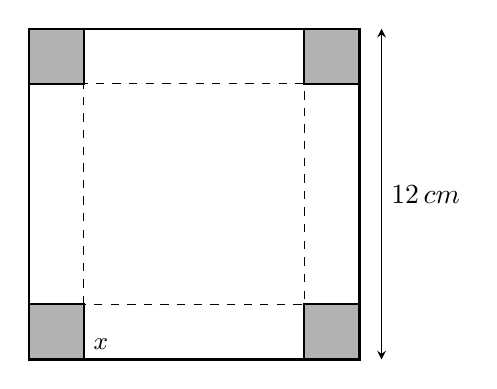
\begin{tikzpicture}[scale=0.35, >=stealth]
    % --- HÌNH 1: MẢNH CÁC TẤM BÌA PHẲNG ---
    % Khai báo kích thước tổng thể và cạnh cắt x
    \def\a{12}
    \def\x{2}
    
    % Tô màu xám cho 4 góc bị cắt
    \fill[gray!60] (0,0) rectangle (\x,\x);
    \fill[gray!60] (0,\a-\x) rectangle (\x,\a);
    \fill[gray!60] (\a-\x,0) rectangle (\a,\x);
    \fill[gray!60] (\a-\x,\a-\x) rectangle (\a,\a);
    \draw[thick] (0,0) rectangle (\x,\x);
    \draw[thick] (0,\a-\x) rectangle (\x,\a);
    \draw[thick] (\a-\x,0) rectangle (\a,\x);
    \draw[thick] (\a-\x,\a-\x) rectangle (\a,\a);
    % Vẽ biên ngoài hình vuông lớn
    \draw[thick] (0,0) rectangle (\a,\a);
    \draw[dashed] (\x,\x) rectangle (\a-\x,\a-\x);
   
    % Kí hiệu đoạn x ở góc
    \node at (\x, 0) [above right] {\small $x$};
    
    % Kí hiệu kích thước cạnh 12cm
    \draw[<->] (\a + 0.8, 0) -- (\a + 0.8, \a) node[midway, right] {$12\,cm$};
\end{tikzpicture}
\quad \quad \quad
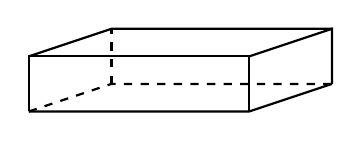
\begin{tikzpicture}[scale=0.35, >=stealth]
    % --- HÌNH 2: HÌNH HỘP CHỮ NHẬT 3D KHÔNG NẮP ---
    % Định nghĩa các điểm tọa độ mặt đáy
    \coordinate (A) at (0,0);
    \coordinate (B) at (8,0);
    \coordinate (C) at (11,1);
    \coordinate (D) at (3,1);
    
    % Chiều cao hộp h
    \def\h{2}
    
    % Các điểm mặt trên
    \coordinate (A1) at (0,\h);
    \coordinate (B1) at (8,\h);
    \coordinate (C1) at (11,3);
    \coordinate (D1) at (3,3);
    
    % Vẽ các nét khuất (nét đứt phía sau)
    \draw[dashed, thick] (A) -- (D) -- (C);
    \draw[dashed, thick] (D) -- (D1);
    
    % Vẽ các nét thấy phía trước và mặt trên mở
    \draw[thick] (A) -- (B) -- (C);
    \draw[thick] (A) -- (A1) -- (B1) -- (B);
    \draw[thick] (B1) -- (C1) -- (C);
    \draw[thick] (A1) -- (D1) -- (C1);
    
\end{tikzpicture}
\end{center}
}{
    \begin{tasks}(4)
        \task \( x = 6 \)
        \task \( x = 3 \)
        \task \( x = 2 \)
        \task \( x = 4 \)
    \end{tasks}
}

% --- CÂU 7 ---
\questionTrueFalse{0}{7}{Một chiếc xe đang chuyển động trên một trục số nằm ngang, gốc O, với chiều dương từ trái sang phải, theo quy luật:

\[s(t) = 3,28t^3 - 9,84t^2 - 78,72t + 32,8,\]

trong đó \( s(t) \) (đơn vị: mét) là vị trí của chiếc xe sau \( t \) giây kể từ khi bắt đầu chuyển động.}{
    \textbf{a)} & Sau 8 giây tính từ lúc bắt đầu chuyển động, chiếc xe cách gốc O một khoảng bằng \( 452,64 \, m \).
    & \textcolor{amberorange}{$\bigcirc$} & \textcolor{amberorange}{$\bigcirc$} \\ \hline
    
    \textbf{b)} & Vận tốc tức thời của chiếc xe tại giây thứ 6 tính từ lúc bắt đầu chuyển động là \( 144,57 \, m/s \).
    & \textcolor{amberorange}{$\bigcirc$} & \textcolor{amberorange}{$\bigcirc$} \\ \hline
    
    \textbf{c)} & Gia tốc của chiếc xe tại thời điểm \( t \) (giây) được tính bằng công thức \( a(t) = 19,68(t - 1) \, (m/s^2) \).
    & \textcolor{amberorange}{$\bigcirc$} & \textcolor{amberorange}{$\bigcirc$} \\ \hline
    
    \textbf{d)} & Trong khoảng thời gian 5 giây tính từ lúc bắt đầu chuyển động, chiếc xe đạt tốc độ lớn nhất tại thời điểm \( t = k \) (giây). Khi đó \( k \) là một số nguyên tố.
    & \textcolor{amberorange}{$\bigcirc$} & \textcolor{amberorange}{$\bigcirc$} \\
}

% --- CÂU 8 ---
\questionTrueFalse{0}{8}{Các bạn học sinh lớp 12A5 muốn làm một tờ báo tường hình chữ nhật. Biết rằng tờ báo tường này phải có diện tích là \( 4 \, m^2 \), và các kích thước của tờ báo tường phải được tối ưu sao cho chu vi của tờ báo là nhỏ nhất. Gọi \( x \) là độ dài một kích thước của tờ báo tường này (\( x \) được tính bằng mét, \( 0 < x < 4 \)).}{
    \textbf{a)} & Độ dài kích thước còn lại của tờ báo tường là \( \dfrac{2}{x} \, (m) \).
    & \textcolor{amberorange}{$\bigcirc$} & \textcolor{amberorange}{$\bigcirc$} \\ \hline
    
    \textbf{b)} & Chu vi của tờ báo tường được cho bởi công thức \( P(x) = 2\left[x + (2 - x)\right] \, (m) \).
    & \textcolor{amberorange}{$\bigcirc$} & \textcolor{amberorange}{$\bigcirc$} \\ \hline
    
    \textbf{c)} & Khi \( x = 0,5 \, m \), chu vi của tờ báo tường này là \( 8,5 \, m \).
    & \textcolor{amberorange}{$\bigcirc$} & \textcolor{amberorange}{$\bigcirc$} \\ \hline
    
    \textbf{d)} & Chu vi nhỏ nhất của tờ báo tường là \( a \, (m) \), khi đó \( 2a + 7 > 22 \).
    & \textcolor{amberorange}{$\bigcirc$} & \textcolor{amberorange}{$\bigcirc$} \\
}

% --- CÂU 9 ---
\questionTrueFalse{0}{9}{Tỉ giá hối đoái giữa hai tiền tệ là tỉ giá mà tại đó một đồng tiền này sẽ được trao đổi cho một đồng tiền khác. Giả sử giá trị của một đồng X, quy đổi theo đồng Y trong khoảng từ năm 2000 đến năm 2010 được tính xấp xỉ bởi công thức \( f(t) = 0,00316t^3 - 0,0471t^2 + 0,114t + 1,47 \), với \( t \) là số năm kể từ năm 2000.}{
    \textbf{a)} & Vào đầu năm 2008, một đồng X có giá trị gần bằng 0,986 đồng Y (làm tròn kết quả đến hàng phần nghìn).
    & \textcolor{amberorange}{$\bigcirc$} & \textcolor{amberorange}{$\bigcirc$} \\ \hline
    
    \textbf{b)} & Đạo hàm của hàm số \( f(t) \) là \( f'(t) = 0,00316t^2 - 0,0471t + 0,114 \).
    & \textcolor{amberorange}{$\bigcirc$} & \textcolor{amberorange}{$\bigcirc$} \\ \hline
    
    \textbf{c)} & Phương trình \( f'(t) = 0 \) có đúng một nghiệm nằm trong khoảng \( (0; 10) \).
    & \textcolor{amberorange}{$\bigcirc$} & \textcolor{amberorange}{$\bigcirc$} \\ \hline
    
    \textbf{d)} & Trong khoảng từ năm 2000 đến năm 2010, một đồng X khi quy đổi theo đồng Y đạt giá trị lớn nhất vào khoảng cuối tháng 4 năm 2001.
    & \textcolor{amberorange}{$\bigcirc$} & \textcolor{amberorange}{$\bigcirc$} \\
}

% --- CÂU 10 ---
\questionTrueFalse{0}{10}{Vào mùa hè, mức độ hoạt động của một chúng loại thần lẫn thay đổi tương ứng với thời gian trong ngày. Một nhà sinh vật học nhận thấy rằng mức độ hoạt động của chúng loại thần lẫn này được mô hình hóa bởi hàm số \( a(t) = 0,008t^3 - 0,288t^2 + 2,304t + 7 \), với \( t \) là số giờ trong ngày tính từ lúc 12 giờ trưa (\( 0 \leq t \leq 24 \)).}{
    \textbf{a)} & Mức độ hoạt động của chúng loại thần lẫn này vào lúc 20 giờ là 1,88.
    & \textcolor{amberorange}{$\bigcirc$} & \textcolor{amberorange}{$\bigcirc$} \\ \hline
    
    \textbf{b)} & Đạo hàm của hàm số \( a(t) \) là \( a'(t) = 0,024t^2 - 0,576t + 2,304 \).
    & \textcolor{amberorange}{$\bigcirc$} & \textcolor{amberorange}{$\bigcirc$} \\ \hline
    
    \textbf{c)} & \( a(15) < a(16) \).
    & \textcolor{amberorange}{$\bigcirc$} & \textcolor{amberorange}{$\bigcirc$} \\ \hline
    
    \textbf{d)} & Mức độ hoạt động của chúng loại thần lẫn này lần lượt đạt giá trị lớn nhất và giá trị nhỏ nhất tại các thời điểm \( t = m \) và \( t = n \). Khi đó, tích \( mn \) là một số chia hết cho 12.
    & \textcolor{amberorange}{$\bigcirc$} & \textcolor{amberorange}{$\bigcirc$} \\
}

% --- CÂU 11 ---
\questionShortAnswer{0}{11}{Tổng doanh thu của một cửa hàng kẹo khi bán được \( x \) trăm gói kẹo được mô tả bởi hàm số  
\[ P(x) = -x^3 + 10x^2 - 12x \]  
(với \( P(x) \) được tính bằng triệu đồng). Khi tổng doanh thu của cửa hàng kẹo này là lớn nhất thì mỗi gói kẹo có giá là bao nhiêu nghìn đồng?}

% --- CÂU 12 ---
\questionShortAnswer{0}{12}{Khi máu đi chuyển từ tim qua các động mạch chính rồi đến các mao mạch và quay trở lại qua các tĩnh mạch, huyết áp tâm thu (tức là áp lực của máu lên động mạch khi tim bóp) liên tục giảm xuống. Giả sử một người có huyết áp tâm thu \( P \) (tính bằng mmHg) được cho bởi hàm số  
\[P(t) = \dfrac{25t^2 + 125}{t^2 + 1}, \quad 0 \leq t \leq 10,\]
trong đó thời gian \( t \) được tính bằng giây. Tính tốc độ thay đổi của huyết áp sau 5 giây kể từ khi máu rời tim.}

% --- CÂU 13 ---
\questionShortAnswer{0}{13}{Chủ của một cửa hàng tạp hóa đã tính toán chi phí để bảo quản và lưu trữ \( x \) lon nước ngọt. Chi phí bảo quản và lưu trữ \( x \) lon nước ngọt này có thể được mô hình hóa bởi hàm số  
\[C(x) = 3x + \dfrac{20000}{x} \quad (\text{với } C(x) \text{ được tính bằng nghìn đồng}).\]
Biết rằng chủ cửa hàng tạp hóa chỉ có thể nhập về tối đa 200 lon nước ngọt mỗi đợt. Hỏi chủ cửa hàng này nên nhập về bao nhiêu lon nước ngọt mỗi đợt để chi phí bảo quản và lưu trữ được tối ưu nhất (tức là đạt giá trị nhỏ nhất)?}

% --- CÂU 14 ---
\questionShortAnswer{0}{14}{Tổng chi phí để vận hành một chiếc xe tải trên một đoạn đường với vận tốc \( v \) (km/h), được cho bởi công thức \( C(v) = 125 + v + \dfrac{4500}{v} \) (với \( C(v) \) được tính bằng chục nghìn đồng). Biết rằng chi phí vận hành thấp nhất của xe tải là \( a \) triệu đồng, và chi phí này đạt được khi vận tốc của xe tải là \( b \) (km/h). Giá trị của \( 2025a + b \) bằng bao nhiêu? (Kết quả làm tròn đến hàng đơn vị).}

% --- CÂU 15 ---
\questionShortAnswer{0}{15}{Giả sử nồng độ thuốc (được tính bằng \( \dfrac{mg}{cm^3} \)) của một loại thuốc giảm đau sau \( t \) giờ kể từ khi được tiêm vào người bệnh được mô hình hóa bởi hàm số \( C(t) = \dfrac{t^2}{2t^3 + 1} \). Biết rằng nồng độ thuốc đạt giá trị lớn nhất bằng \( \dfrac{m}{n} \) \( mg/cm^3 \) là phân số tối giản, \( m, n \in \mathbb{N}^* \) vào thời điểm \( p \) giờ, và sau một thời gian dài, nồng độ thuốc trong người bệnh sẽ tiến đến \( 0 \, mg/cm^3 \). Giá trị của \( m + 2n + 3p + 4q \) bằng bao nhiêu?}

\end{document}